\documentclass[12pt]{article}

% Packages
\usepackage{amsmath, amssymb, amsthm}
\usepackage{geometry}
\usepackage{graphicx}
\usepackage{tikz}
\usepackage{hyperref}
\usepackage{titlesec}

\geometry{margin=1in}

\title{Generative Theory: The Renji-$\Omega$ Framework}
\author{Renji Nakayama}
\date{January 2026}

\begin{document}

\maketitle

\begin{abstract}
This paper presents the foundational structure of Generative Theory, a unified framework describing how worlds, structures, and selves emerge from an undifferentiated field $\Omega$ through directional generation (F), stability landscapes ($\Phi$), generative flows (G), spectral fluctuations (S), and recursive hierarchical formation. The Renji-$\Omega$ framework provides the minimal generative basis for understanding the emergence of space, time, matter, world-models, and consciousness.
\end{abstract}

\tableofcontents
\newpage

% ---------------------------------------------------------
\section{Introduction}

Generative Theory (Renji Generative Theory) aims to reconstruct the emergence of the world from first principles, without assuming space, time, particles, or laws as given. Instead, the world is treated as a generative process:

\[
\Omega \rightarrow F \rightarrow \Phi \rightarrow G \rightarrow S \rightarrow \text{point} \rightarrow \text{space} \rightarrow \text{structure} \rightarrow \text{world model} \rightarrow \text{self model} \rightarrow \text{consciousness}.
\]

This document provides the formal structure of the Renji-$\Omega$ framework.

% ---------------------------------------------------------
\section{$\Omega$: The Undifferentiated Field}

The Renji-$\Omega$ structure represents a fully symmetric, undifferentiated field:

\begin{itemize}
\item no direction
\item no distance
\item no time
\item no particles
\item no space
\end{itemize}

Yet it is not ``nothing.''

It is a field of maximal generative potential, capable of symmetry breaking.

% ---------------------------------------------------------
\section{F: Four Generative Directions}

When $\Omega$ undergoes minimal symmetry breaking, four irreducible generative directions emerge:

\begin{center}
\begin{tabular}{c|c|c}
Direction & Meaning & Role \\
\hline
Dir & Local coherence & Proto-particle formation \\
Ent & Spreading / equalization & Proto-wave behavior \\
Was & Transport / distance & Proto-geometry \\
His & Temporal consistency & Proto-time / causality \\
\end{tabular}
\end{center}

These four directions form the minimal generative basis.

% ---------------------------------------------------------
\section{$\Phi$: Stability Landscape (10 Components)}

Repeated application of F produces a stability landscape $\Phi$ with 10 components:

\subsection{Pure components}

\[
\Phi_{\text{Dir}},\ \Phi_{\text{Ent}},\ \Phi_{\text{Was}},\ \Phi_{\text{His}}
\]

\subsection{Interaction components}

\[
\Phi_{\text{Dir--Ent}},\
\Phi_{\text{Dir--Was}},\
\Phi_{\text{Dir--His}},\
\Phi_{\text{Ent--Was}},\
\Phi_{\text{Ent--His}},\
\Phi_{\text{Was--His}}
\]

$\Phi$ is not an energy function but a measure of generative naturalness.

% ---------------------------------------------------------
\section{G: Generative Flow}

Given the stability landscape, the world begins to move along its natural gradients:

\[
G = -\sum_{i=1}^{10} \nabla \Phi_i.
\]

This multi-directional gradient flow drives the world from unstable to stable configurations.

% ---------------------------------------------------------
\section{S: Proto-Wave Spectrum}

Linearizing $G$ near stable points yields eigenvalues and eigenvectors:

\[
DG(x_0) v = \lambda v.
\]

The imaginary components of $\lambda$ produce oscillatory modes:

\begin{itemize}
\item Dir--Ent balance $\rightarrow$ oscillation (wave behavior)
\item His coupling $\rightarrow$ interference (non-Markovian)
\item Was ambiguity $\rightarrow$ nonlocality
\end{itemize}

S represents the ``wave of possibilities'' before solidification.

% ---------------------------------------------------------
\section{Hierarchical Phase Transitions}

\subsection{S $\rightarrow$ point (Dir)}
Local coherence produces discrete, stable modes.

\subsection{point $\rightarrow$ space (Was)}
Distances and configurations emerge.

\subsection{space $\rightarrow$ structure (His)}
Spatial patterns persist over time.

\subsection{structure $\rightarrow$ next level (recursion)}
Structures become points at the next level:

\[
L_{n+1} = \text{Stabilize}(\text{Arrange}(L_n)).
\]

This recursion generates arbitrarily deep hierarchies.

% ---------------------------------------------------------
\section{World Model}

A world model is a compressed representation of hierarchical structure:

\begin{itemize}
\item objects
\item relations
\item persistence
\end{itemize}

It is not a copy of the external world but an internal generative interpretation.

% ---------------------------------------------------------
\section{Self Model}

The self model operates on the world model:

\begin{itemize}
\item referencing it
\item updating it
\item treating it as ``mine''
\end{itemize}

This produces the first form of agency.

% ---------------------------------------------------------
\section{Consciousness}

Consciousness emerges when:

\[
\text{world model} \leftrightarrow \text{self model}
\]

form a stable recursive loop, temporally aligned by His.

Consciousness is thus a generative, recursive, self-updating process.

% ---------------------------------------------------------
\section{Generative Flow Diagram (TikZ)}

\begin{center}
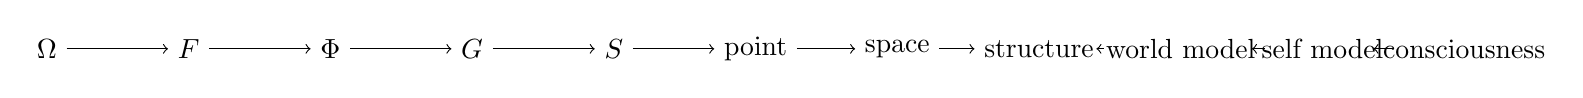
\begin{tikzpicture}[node distance=1.8cm, auto]
\node (o) {$\Omega$};
\node (f) [right of=o] {$F$};
\node (phi) [right of=f] {$\Phi$};
\node (g) [right of=phi] {$G$};
\node (s) [right of=g] {$S$};
\node (p) [right of=s] {point};
\node (sp) [right of=p] {space};
\node (st) [right of=sp] {structure};
\node (wm) [right of=st] {world model};
\node (sm) [right of=wm] {self model};
\node (c) [right of=sm] {consciousness};

\draw[->] (o) -- (f);
\draw[->] (f) -- (phi);
\draw[->] (phi) -- (g);
\draw[->] (g) -- (s);
\draw[->] (s) -- (p);
\draw[->] (p) -- (sp);
\draw[->] (sp) -- (st);
\draw[->] (st) -- (wm);
\draw[->] (wm) -- (sm);
\draw[->] (sm) -- (c);
\end{tikzpicture}
\end{center}

% ---------------------------------------------------------
\section*{Author Information}

Renji Nakayama \\
Creator of the Renji-$\Omega$ Generative Framework \\
Tokyo, Japan \\
January 2026

\end{document}